% ------------------------------------------------------------------------------
%
% PREAMBLE
%
% ------------------------------------------------------------------------------

\documentclass[12pt, titlepage]{article}


\usepackage{graphicx, amsmath, amssymb, natbib, setspace, sectsty, verbatim, 
		mathrsfs, float}
\usepackage{MnSymbol}
\usepackage{multirow}
\usepackage{bm}
\usepackage[usenames, dvipsnames]{color}
\bibpunct{(}{)}{;}{a}{}{,}
\setlength{\parindent}{3em}
%\parskip = 1.5ex
%\linespread{1.3}
%\onehalfspacing

\pdfpagewidth 8.5in
\pdfpageheight 11in
\setlength{\oddsidemargin}{0.0in} \setlength{\textwidth}{6.5in}
\setlength{\topmargin}{0.15in} \setlength{\textheight}{8.5in}
\setlength{\headheight}{0.0in} \setlength{\headsep}{0.0in}

\usepackage{/mnt/ExtraDrive1/Work/shTex/mymacros}

\providecommand{\norm}[1]{\lVert#1\rVert}
\newcommand{\csection}[1]{\section[#1]{\centering #1 }}
\subsectionfont{\small}
\newcommand{\cye}[1]{\color{yellow!70!black}#1}
\newcommand{\cre}[1]{\color{red!70!black}#1}
\newcommand{\cbl}[1]{\color{blue!70!black}#1}
\newcommand{\cgr}[1]{\color{green!70!black}#1}


% ------------------------------------------------------------------------------
%
% BEGIN DOCUMENT
%
% ------------------------------------------------------------------------------

\begin{document}

\setcounter{equation}{0}
\renewcommand{\theequation}{R.\arabic{equation}}


% ------------------------------------------------------------------------------
%
%                       Section 9.10.1
%          Prediction of trends in harbor seal abundance
%
% ------------------------------------------------------------------------------


\vspace{.3cm}

{\large \flushleft \textbf{9.10.1 Prediction of trends in harbor seal abundance}}

\vspace{.3cm}

We continue with our analysis from Section 8.8.1 of the trends in harbor seal abundance in southeast Alaska.  In Chapter 8, we made inferences on covariance parameters and fixed effects.  Here, our inferential goal will be to make prediction, with prediction intervals, for sites with missing data, and also to investigate leave-one-out cross-validation (LOOCV) as a way to smooth autoregressive models.

Recall from the Chapter 8 harbor seal example that we discussed some computational issues when there are missing data for the spatial-weights models.  We were able to obtain the inverse of the covariance matrix for the observed sites, which we called $\boldsymbol{\Sigma}_{oo}^{-1}$, from the inverse covariance matrix for all sites with an inverse whose dimensions were those of the \textit{missing} data.  For estimation of covariance parameters, and fixed effects, this was enough.  However, for prediction, we also need $\boldsymbol{\Sigma}_{ou}$ and $\boldsymbol{\Sigma}_{uu}$ from the full covariance matrix (not its inverse), because, in the notation of Chapter 9, we need $\mathbf{R}^{-1}\mathbf{R}_{\mathbf{y}\mathbf{u}}$ and $\mathbf{R}_{\mathbf{u}\mathbf{u}}$ (see Section 9.1). It is possible to obtain $\mathbf{R}^{-1}\mathbf{R}_{\mathbf{y}\mathbf{u}}$ by noting that $\boldsymbol{\Sigma}_{oo}^{-1}\boldsymbol{\Sigma}_{ou} = -\boldsymbol{\Sigma}^{ou} (\boldsymbol{\Sigma}^{uu})^{-1}$ and we may have already computed $(\boldsymbol{\Sigma}^{uu})^{-1}$ for likelihood evaluations and estimation of covariance parameters and fixed effects.  However, for $\boldsymbol{\Sigma}_{uu}$, we need another inverse. We have $\boldsymbol{\Sigma}_{oo}^{-1}$, but need to take its inverse to obtain $\boldsymbol{\Sigma}_{oo}$ by noting that $\boldsymbol{\Sigma}_{uu} = (\boldsymbol{\Sigma}^{uu})^{-1} + (\boldsymbol{\Sigma}^{uu})^{-1}\boldsymbol{\Sigma}^{uo} \boldsymbol{\Sigma}_{oo}\boldsymbol{\Sigma}^{ou} (\boldsymbol{\Sigma}^{uu})^{-1}$.  Note that we only need to obtain $\boldsymbol{\Sigma}_{oo}$ once for prediction, while $\boldsymbol{\Sigma}_{oo}^{-1}$ needs repeated evaluations during likelihood optimization.

{\large \center \textbf{ ------ start LOOCV and n-fold ---------}}
\vspace{.3cm}

[Dale, the following is the same description of LOOCV that I wrote for the wet sulfate data.  I think that this description, along with n-fold cross-validation, could be a topic in Chapter 9 apart from the examples, as I will likely refer to them for all of the examples.  I will leave this here for now.  Please feel free to re-organize.]


LOOCV eliminates one datum at a time, using all of the rest of the data to predict the one that was removed.  There is a fast and a slow way to do this.  The slow way is to remove a datum and then re-estimate all of the parameters using ML or REML estimation each time.  However, with the removal of but a single datum, the parameter estimates change very little.  A fast way to achieve LOOCV is based on holding all parameters at their values as estimated by using all of the data, and then using results from partitioned matrices so that we only have to invert the covariance matrix once (which can be saved from the ML or REML estimation, so there is in fact no additional matrix inverses are required).  Recall from Section 5.6 that,
if a matrix is partitioned as,
$$
    \boldsymbol{\Sigma} = 
    \begin{bmatrix}
       \boldsymbol{\Sigma}_{11} & \boldsymbol{\Sigma}_{12} \\
       \boldsymbol{\Sigma}_{21} & \boldsymbol{\Sigma}_{22}
    \end{bmatrix}  \ \textrm{ and } \  
    \bSigma^{-1} = 
    \begin{bmatrix}
       \boldsymbol{\Sigma}^{11} & \boldsymbol{\Sigma}^{12} \\
       \boldsymbol{\Sigma}^{21} & \boldsymbol{\Sigma}^{22}
    \end{bmatrix}, 
$$
then 
$$
    \boldsymbol{\Sigma}_{11}^{-1} = \boldsymbol{\Sigma}^{11} - \boldsymbol{\Sigma}^{12} (\boldsymbol{\Sigma}^{22})^{-1} \boldsymbol{\Sigma}^{21}.
$$
Moreover, let us order the data such that the datum to be removed is last, so that $\boldsymbol{\Sigma}^{22}$ is a scalar, then the inverse of $\boldsymbol{\Sigma}^{22}$ is trivial and $\bSigma_{11} \upi$ can be computed rapidly. The main computational expense of kriging predictions rely on the inverse covariance matrix for the observed data, but in LOOCV that is given by $\bSigma_{11} \upi$, which is computed rapidly without any further matrix inverses if we already have $\bSigma \upi$. The only other quantity from $\boldsymbol{\Sigma}$ needed for prediction is the vector $\boldsymbol{\Sigma}_{12}$.  Conceptually, we just re-order the data, one at a time, putting the one to be removed last in the covariance matrices above, and that allows the predictions to be computed quickly.

Let $\hat{y}_{i} = \bar{u}$ from (9.2) be the $i$th predicted value using LOOCV where the $i$th datum has been removed, and let $\hat{v}_{i} = \sqrt{\var(\bar{u} - u)}$ from (9.3) be the $i$ prediction standard error.  Then we will consider two metrics to assess model performance.  One is the root-mean-squared prediction error (RMSPE), which we computed as
$$
\sqrt{\frac{1}{n}\sum_{i=1}^{n} (\hat{y}_{i} - y_{i})^{2} }.
$$
Models with lower RMSPE have better predictive performance.  The other metric is the 90\% prediction interval coverage, PIC90, which we computed as
$$
\frac{1}{n} \sum_{i=1}^{n} \mathcal{I}(\hat{y}_{i} - z_{1-\alpha/2}v_{i} \le y_{i} \le \hat{y}_{i} + z_{1-\alpha/2}v_{i}),
$$
where $\mathcal{I}(\cdot)$ is an indicator function, equal to 1 if its argument is true, and 0 otherwise, and $z_{1-\alpha/2}$ is a standard normal value below which contains $1-\alpha/2$ of the probability density.  We chose $\alpha = 0.1$ for PIC90, resulting in the familiar $z_{0.95} = 1.645$.

One problem with LOOCV is that it may be overly optimistic in assessing actual prediction.  A simple thought experiment reveals why.  Suppose 99 data locations were clustered very closely together, and another was separated from the cluster.  Then, for LOOCV, as we removed each datum from the cluster, we would have many nearby locations and get very precise predictions with small prediction standard errors, and they would swamp RMSPE and PIC90 if our overall goal was to predict in a region that was substantially larger than that enclosing the cluster of locations. The same is essentially true if all locations were pairs of locations that were very close to each other, but the pairs were scattered.  Still, under normal sampling scenarios, it can be a good way to evaluate models as they are all operating under the same sampling scheme.

A second way to use cross-validation is called $n$-fold cross-validation.  Here we divide the data into $n$ groups, and remove one whole group to be predicted -- this is often called the \textit{test} dataset.  The remaining data are called the \textit{training} dataset, and are used to fit a model and make predictions at the locations of the test dataset.  Then, the predictions at the locations for the test dataset can be compared to the actual values that were removed.  In fact, RMSPE and PIC90 can be computed for $n$-fold cross-validation in exactly the same way as for LOOCV, and to distinguish them, we use RMSPE$_{\textrm{Lo}}$ and PIC90$_{\textrm{Lo}}$ for LOOCV, and RMSPE$_{\textrm{Nf}}$ and PIC90$_{\textrm{Nf}}$ for $n$-fold cross-validation. With $n$-fold cross-validation we do not have to fit the model as many times, so we completely re-fit the model for each group that is removed.  Groups are often created randomly, and we will do it this way too.  If we want to get the best feel how well a model will interpolate, that includes even a bit of extrapolation at the edges, it is desirable to have just a few groups.  This may be more pessimistic about model performance than the real data because we are decreasing our sample sizes substantially.  Nevertheless, to examine both extremes, where LOOCV is overly optimistic, we used 3-fold cross-validation, which is overly pessimistic.  Because we created 3 groups randomly, we would like to ensure that our results do not depend too much on any particular randomized grouping.  Hence, we do 3-fold cross-validation 10 times, and average the results for RMSPE (by first averaging the mean-squared prediction error, and then taking the square root) and PIC90.

{\large \center \textbf{ ------ end LOOCV and n-fold ---------}}
\vspace{.3cm}

Based on our evaluation of likelihoods in Section 8.8.1, CAR models with row-standardization appeared much better than SAR models and models without row-standardization.  It also appeared that the model with isolated sites, at the cost of an extra parameter, was better than any of those where all sites were forced to be connected.  Does this translate to predictive performance?  We investigated using LOOCV. All models discussed will contain the stock effect unless otherwise noted and are estimated with REML. The CAR row-standardized covariance with islands (three covariance parameters) was still best, based on LOOCV RMSPE, with a value of 0.01739.  This was followed by the same model without row standardization with RMSPE = 0.01751.  A CAR covariance model without islands, based on a first-order neighbor structure, was next with RMSPE = 0.01765, but the same model with a fourth-order neighbor structure did very poorly with RMSPE = 0.02775, even though this was the best model in Figure~\ref{Fig:Seals_m2LLAIC}B according to AIC.  This reinforces the idea that a variety of model checks should be performed before settling on any one model, and it can be difficult to come to a decision when different criteria identify different ``best'' models.  A model without any spatial autocorrelation, assuming uncorrelated random errors, had RMSPE = 0.01777.  Finally, we tried a model based purely on spatial autocorrelation, without any fixed effects except a constant mean, and a CAR row-standardized covariance with islands, that resulted in RMSPE = 0.01800.

Based on these results, we feel confident in proceeding with the CAR row-standardized covariance with islands.  An important inference concerning these data was about the effect of genetic stock on trend, which was explored in Chapter 8.8.1, but now we would also like to predict values for missing data, and make smoothed maps of the existing data.  To explain smoothing, Figure~\ref{Fig:seals_predhisto}A shows a histogram of the observed values and the LOOCV values.  It is possible for predictions to be more extreme than observed values, but here, with a covariate effect of group means, and fairly weak autocorrelation, predictions ``shrink'' away from extremes.  LOOCV predictions are a combination of the estimated stock mean plus and a weighted average of local residuals, which causes the predictions to be much less variable than the original data.  Predictions of the missing data are presented in Figure~\ref{Fig:seals_predhisto}B. For the independence model, the predictions can take on only one of five possible values, which are the five estimated stock means, shown by the darkest black bars.  Predictions for the pure mean model, without the stock effect, are shown, as well as those with the stock effect.  When spatial autocorrelation is included in the model with stock effect, the predictions can take on values that deviate from the stock means because they include weights from the residuals of neighboring sites in the same way that they did for LOOCV.  Broadly speaking, the spreads of the predictions are roughly similar for the mean-only model and the one that includes the stock effect, and they are very similar to the spread of the LOOCV predictions.  LOOCV, combined with prediction of missing data, is one way to smooth maps, but there are many others.  Here, we will use LOOCV.
\begin{figure}[H]
  \begin{center}
	    \includegraphics[width=.9\linewidth]{seal_predhist}
  \end{center}
  \caption{Histograms of raw data and predictions. A. Darker shaded histogram is laid over the histogram of the raw data in a lighter shade.  B. Histograms of predictions for three different models.  The darkest shade is a stock effect model assuming independent errors.  The middle shade has autocorrelated errors, but a single mean effect.  The lightest shade has stock effects in the model, along with autocorrelated errors. \label{Fig:seals_predhisto}}
\end{figure}

Figure~\ref{Fig:seal_maps}A show predictions for all 159 site with missing values.  These are shown as colored circles, and are superimposed on the colored polygons of raw values. Notice that the range of values, given by the legend, are the same as the range for the raw values in Figure~\ref{Fig:seals_predhisto}.  The prediction standard errors (Figure~\ref{Fig:seal_maps}B) are highest near the edges where sites have fewer neighbors, as we expect from the row-standardized model.  On occasion, high standard errors occur for interior sites because it is possible for them to have few neighbors.  The predictions of missing data, along with LOOCV values for locations with raw data, are given in Figure~\ref{Fig:seal_maps}C.  Notice (from the legend) that the range of values is much narrower than Figure~\ref{Fig:seal_maps}A, and this qualifies as a smoothed map.  The effect of stock mean is fairly evident in Figure~\ref{Fig:seal_maps}C. As in Figure~\ref{Fig:seal_maps}B, the prediction standard errors (Figure~\ref{Fig:seal_maps}D) are highest near the edges where sites have fewer neighbors. Figure~\ref{Fig:seal_maps}E show predictions of missing data, along with LOOCV, for for the same covariance model as previously, but without the stock effects (a common mean).  Notice that this is also a smoothed map with slightly more range in values than the stock-effect model, and the effect of stock is not as evident.  The standard error map (Figure~\ref{Fig:seal_maps}F) looks very similar to the other standard error maps.

\begin{figure}[H]
  \begin{center}
	    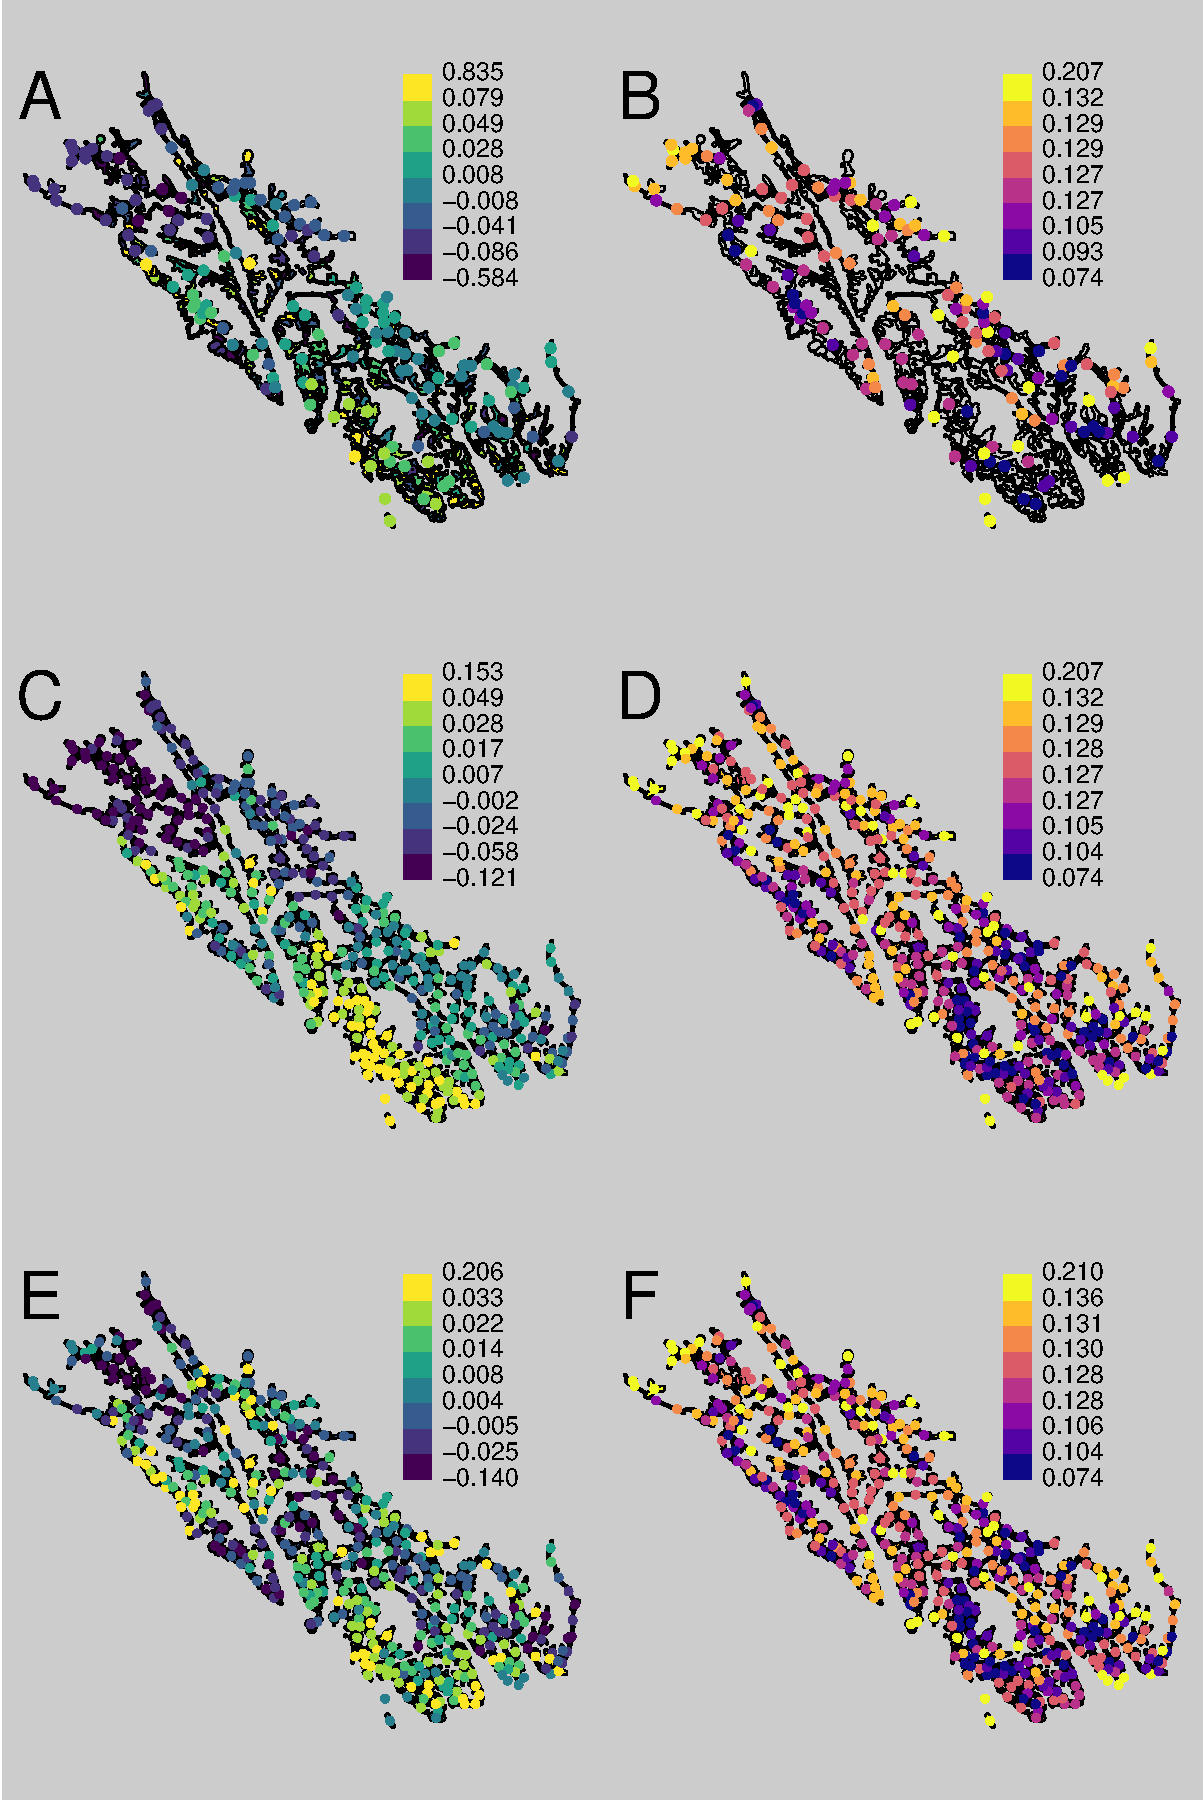
\includegraphics[width=.75\linewidth]{seal_maps}
  \end{center}
  \caption{Prediction maps (left column) and prediction standard errors (right column) for a variety of models. A-B Model includes stock effect, and a row-standardized CAR model with islands (no neighbors, resulting in an extra parameter). C-D LOOCV, rather than raw values, for the same model, E-F LOOCV and predictions for the same covariance model as above but with a common mean model as the single fixed effect. \label{Fig:seal_maps}}
\end{figure}

%%%%%%%%%%%%%%%%%%%%%%%%%%%%%%%%%%%%%%%%%%%%%%%%%%%%%%%%%%%%%%%%%%%%%%%%%%%%%%%%
%%%%%%%%%%%%%%%%%%%%%%%%%%%%%%%%%%%%%%%%%%%%%%%%%%%%%%%%%%%%%%%%%%%%%%%%%%%%%%%%                BIBLIOGRAPHY
%%%%%%%%%%%%%%%%%%%%%%%%%%%%%%%%%%%%%%%%%%%%%%%%%%%%%%%%%%%%%%%%%%%%%%%%%%%%%%%%
%%%%%%%%%%%%%%%%%%%%%%%%%%%%%%%%%%%%%%%%%%%%%%%%%%%%%%%%%%%%%%%%%%%%%%%%%%%%%%%%

%\bibliographystyle{consbiol}
\bibliographystyle{/mnt/ExtraDrive1/Work/shTex/asa}
\bibliography{DaleChap883.bib}
%\bibliographystyle{/home/jay/Data/shTex/shTex/asa}
%\bibliography{/home/jay/Data/shTex/shTex/StatBibTex.bib}




\end{document}

